\section{Introduction}

\subsection{Context}

The ride-sharing problem is fundamentally about correctly connecting two groups of people. One group is customers, who need a ride from their current position to somewhere else; the other is drivers, each of whom owns a vehicle they can use to take a customer from their origin to their destination. In the past, ride-sharing mostly meant carpooling, in which travellers with a shared origin or destination split the costs of one private vehicle and were matched manually through employer programs or telephone services~\citep{chan2012ridesharing}. Nowadays, the process is much more real-time and complex, as ride-sharing programs have integrated the Internet into their platforms~\citep{chan2012ridesharing}. Ride-sharing platforms use algorithms to assign drivers to customers as efficiently as possible~\citep{agatz2012optimization}. This can mean optimizing potentially thousands of rides each minute.

The ride-sharing problem covers a larger family of problems. Strictly defined, ride-sharing is a trip which has at least two people sharing one vehicle, and any payment collected covers only part of the driver's costs rather than producing a profit~\citep{furuhata2013ridesharing,chan2012ridesharing,mitropoulos2021systematic}. The term is nevertheless used for practices that range from short everyday trips to commuting and long-distance travel~\citep{pigalle2023ridesharing}. Under this broader definition, ride-sharing can mean carpooling, in which several customers share the same vehicle for some part of their trips, or it can mean ride-hailing, in which a driver serves only one customer at a time, and the ride-sharing platform chooses which driver transports which customers. All variants share platform prearrangement, which separates them from hailing a taxi on the street~\citep{furuhata2013ridesharing}. In operations research terms, they belong to the family of pickup-and-delivery problems~\citep{savelsbergh1995general}, and the passenger-carrying special case in which customer convenience matters is known as the dial-a-ride problem~\citep{cordeau2007dialaride}. The problem can also vary depending on what information is available before solving it. For example, we may have all drivers' pickup times and origin and destination locations immediately, or we may receive them dynamically over time, in which case matching must be done automatically on very short notice~\citep{agatz2012optimization,berbeglia2010dynamic}. While the details differ across variations, the core problem remains the same: how to assign a set of customer requests to a set of vehicles. This thesis investigates the ride-hailing variant, in which each customer travels alone and the drivers work fixed shifts for the platform, and a more static version of the problem, in which we know all parameters for each customer before solving, but we solve the drivers' schedules separately.

Solving the problem requires two decisions. First, we need to assign customers to drivers appropriately. Customers may have preferences for the kind of driver or vehicle they would like to travel with. For example, these can include age, gender, vehicle brand, and whether the vehicle is electric. Some preferences can be deal-breakers, meaning a customer will not travel with some driver. Such screening is driven largely by trust between strangers, and folding it into the matching itself is known as high-dimensional matching~\citep{furuhata2013ridesharing,chaube2010trust}. Such preferences directly limit how many matches a system can produce. The number of matches formed grows with the probability that two participants have compatible trips, so the stricter the compatibility, the fewer matches remain~\citep{dailey1999seattle}. Even when participants have a common route, actually finding a suitable match is not easy~\citep{hall1997dynamic}. This thesis considers only customers' preferences and does not consider drivers' preferences. Second, we need to figure out ride timing. Rides must be ordered so, for example, that each customer does not arrive too late at their destination and the driver does not have to travel too far without a customer. These two decisions have well-known mathematical problem definitions. The assignment is a matching problem, for which a large family of algorithms exists~\citep{pentico2007assignment}, and the timing is a scheduling problem. Both are combinatorial problems that are difficult to solve with known methods, and while they are already difficult individually, the decisions also constrain each other: a customer not matched to a driver cannot be scheduled for that driver.

The objective is to find a good-enough compromise between two groups of people with different priorities. Customers want their driver to arrive exactly when they are ready and for the ride itself to be fast, while drivers want to maximise their earnings. These interests must be balanced in a single objective function that typically weighs serving as many customers as possible, keeping operating costs low, and minimising customer inconvenience~\citep {agatz2012optimization,cordeau2007dialaride}.

\begin{figure}[!h]
  \centering
  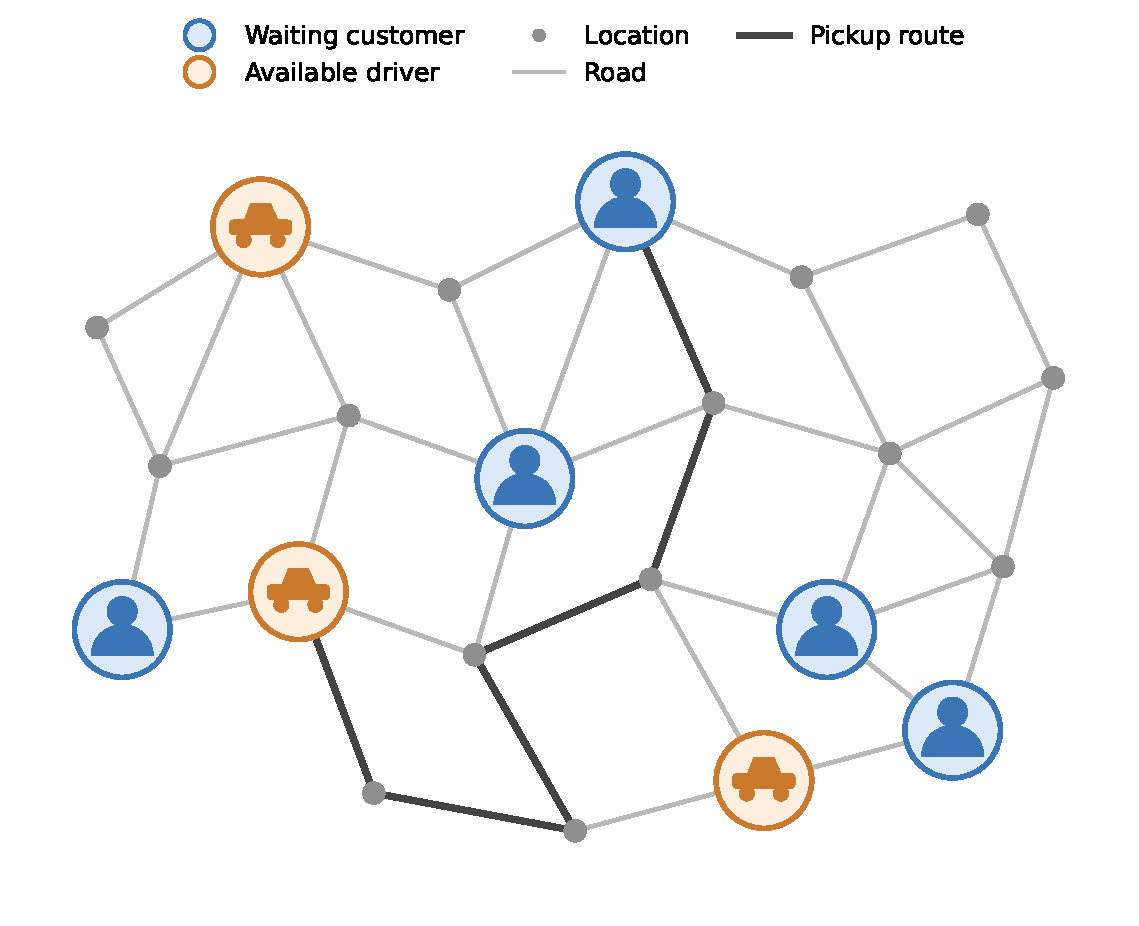
\includegraphics[width=\textwidth]{figures/ridesharing_illustration.pdf}
  \caption{Illustration of the ride-sharing problem}
  \label{fig:ride-sharing-illustration}
\end{figure}

Figure~\ref{fig:ride-sharing-illustration} illustrates the setting in a simple scenario. Customers wait at their pickup locations for a driver to be selected, and drivers wait for rides to be assigned. In reality, hundreds of customers may be waiting at a given moment, along with tens of drivers. Also, the number of locations is much larger in reality.

Simply put, this thesis studies the following problem: each customer provides their desired pickup time, destination location, and a list of drivers they are willing to be assigned to. Each driver has a shift with a fixed start and end time. A solution assigns customers to drivers and then determines the best schedule for each driver. In our problem, not all customers will be served. We measure the solution's performance by how many customers were not served, how long customers waited for pickup after their desired pickup times, and how much of the shift drivers spent idle.

\subsection{Motivation}

Despite having all the technology needed for successful ride-sharing, it has not grown as much as we expected~\citep{chan2012ridesharing}. The share of American workers commuting by carpool fell from 20.4 percent in 1970 to 10.7 percent in 2008~\citep{chan2012ridesharing}. Ride-sharing still accounts for only around 8 percent of trips in Canada and 11 percent in the United States, despite over 600 ride-matching programs operating there~\citep{chan2012ridesharing}. The problem is no longer connecting people, but deciding whom to connect with whom.

First, an algorithm that solves the ride-sharing problem quickly becomes complex, and using it can be time-consuming and possibly expensive. A system that matches thousands of customers to hundreds of drivers must solve a combinatorial optimisation problem constrained by the needs and wants of both groups~\citep{agatz2012optimization}. Also, because a matching system must respond within minutes, possibly seconds, it cannot compute an exact solution, as the classical dynamic programming solution to the single-vehicle dial-a-ride problem already requires computational effort that is exponential in the size of the problem~\citep{psaraftis1980dynamic,agatz2012optimization}. A natural solution is to split the problem into multiple smaller problems that are easier to solve independently, and to accept that the solution might no longer be completely optimal~\citep{agatz2012optimization}. This is a reasonable trade-off, and in this thesis we try an alternative approach to the problem.

Secondly, a solution is only useful if both the customers and drivers accept it. Trust, along with convenience and incentives, determines whether a person participates in a ride-sharing service at all~\citep{chaube2010trust}. Nevertheless, users are usually assumed to perform the screening rather than having it built into the matching~\citep{furuhata2013ridesharing}. Drivers are treated no better, as the objectives used in the literature are mostly system-wide or customer-facing, such as total vehicle-miles, total travel time, or the number of customers served~\citep{furuhata2013ridesharing,agatz2012optimization}. The driver appears mainly as a cost. A model that ignores either the customers or drivers can produce schedules that are optimal in theory but are refused in real-world use.

\subsection{Structure}

The rest of this thesis is organised as follows. Section~\ref{sec:literature-review} reviews the earlier work on ride-sharing and matching problems. Section~\ref{sec:methods} presents the thesis methodology. It introduces the problem statement, the three-step pipeline, the maximum-flow formulation of the matching problem, the integer linear program that schedules every driver, and the conflict-resolution step that ensures each customer is assigned to only one driver. Section~\ref{sec:experimental-settings} describes the synthetic test instances, the parameter values used in all instances, and the final results of each step. Section~\ref{sec:conclusion} summarises the findings, discusses the pipeline and formulation limitations, and outlines possible directions for future research.
